\documentclass[11pt]{article}
\title{How the Codynamic Book Machine Works}
\author{Arthur Petron}
\usepackage[margin=1in]{geometry}
\usepackage{graphicx}
\usepackage{amsmath,amssymb,mathtools}
\usepackage{tikz}
\usetikzlibrary{positioning,arrows.meta}
\usepackage{hyperref}
\graphicspath{{media/}{media/diagrams/}{images/}{artwork/}}

\begin{document}

\section*{Proposals, Diffs, and Review}

In this system, an edit is not treated as an invisible mutation of the manuscript. It is first shaped into a proposal: a bounded change with an author, a target section, a rationale, and a traceable payload. That distinction matters because the book machine is designed to keep authorship legible at every step. A section agent does not silently overwrite text; it produces a section payload that can be inspected, compared, and revised before it becomes part of the durable manuscript state.

A proposal is therefore more than a draft. It is a reviewable unit of work that can carry metadata about where it came from, what task produced it, and which section it affects. In practice, this metadata lets the system distinguish a fresh draft from a later repair pass, a gardener-driven revision, or a callback triggered by another agent. The result is a manuscript history that can be reconstructed from durable records rather than inferred from the latest file contents alone. In other words, the proposal record preserves intent, the payload preserves the text, and the metadata preserves the circumstances under which that text was produced.

Diffs are the mechanism that makes those proposals legible. When a section changes, the system can compare the new payload against the prior version and expose the exact textual delta. That comparison is useful both for human review and for downstream automation. A reviewer can see what changed without rereading the entire section, and an agent can reason about whether the change is local, whether it introduces a new dependency, or whether it should trigger follow-up work in a sibling section. A diff is therefore not just a convenience for editors; it is part of the machine's coordination logic.

Checkpoints provide a second layer of durability. Instead of treating the latest text as the only state that matters, the machine can preserve intermediate versions as named or timestamped milestones. Those checkpoints make it possible to recover from a bad revision, to inspect the evolution of a section over time, and to separate experimental edits from committed ones. In a long-form technical document, that separation is especially valuable because a later repair may need to refer back to an earlier stable state rather than the most recent but still unverified draft. Checkpoints also make revision history easier to audit when a section has passed through several rounds of gardening or callback-driven repair.

This reviewable workflow also supports editorial accountability. A section agent can generate prose, but the prose remains provisional until it has passed through the system's review surfaces: the proposal record, the diff, and any subsequent repair or gardening pass. That means the manuscript is not a stream of opaque writes. It is a sequence of visible decisions, each of which can be attributed to a task, a message, or a callback in the runtime log. The point is not merely to keep a history; it is to keep a history that explains why the text changed.

The same principle applies to coordination between agents. If a gardener identifies a coherence issue, the resulting revision request is itself a durable artifact. If a reference is missing, the section agent does not fabricate support; it routes the need through the reference workflow and waits for a registered key before revising the text. If a diagram would materially improve the section, the request is explicit and the resulting asset is inserted only after the callback arrives. In each case, the system prefers a visible handoff over an implicit side effect. That preference keeps the manuscript's evolution inspectable even when several agents are working at once.

This is why proposals, diffs, and checkpoints belong together. Proposals define intent, diffs expose change, and checkpoints preserve recoverable states. Together they turn agent-authored editing into a reviewable process rather than a hidden mutation pipeline. That design keeps the manuscript inspectable, makes revision history durable, and gives both humans and agents a stable basis for further work. It also aligns this chapter with the surrounding sections: section payloads establish the owned text surface, while compilation and repair loops in the next section will show how those reviewable changes become buildable artifacts.

\begin{figure}[htbp]
\centering
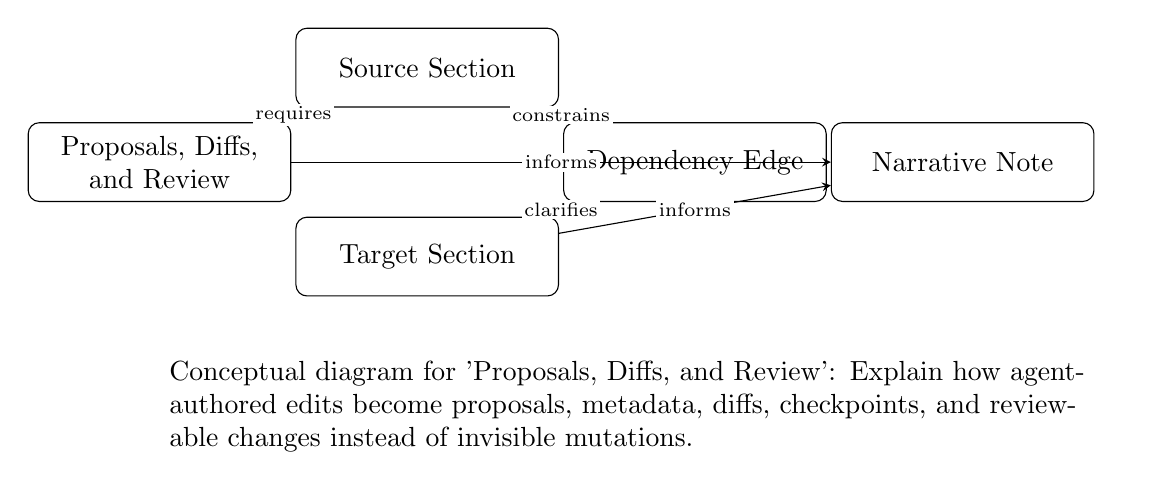
\begin{tikzpicture}[>=stealth, node distance=2.2cm,
  concept/.style={draw, rounded corners, align=center, text width=3.1cm, minimum height=1cm},
  relation/.style={font=\scriptsize, fill=white, inner sep=1pt}]
\node[concept] (n1) at (0,0) {Proposals, Diffs, and Review};
\node[concept] (n2) at (3.4,1.2) {Source Section};
\node[concept] (n3) at (6.8,0) {Dependency Edge};
\node[concept] (n4) at (3.4,-1.2) {Target Section};
\node[concept] (n5) at (10.2,0) {Narrative Note};
\draw[->] (n1) -- node[relation] {requires} (n2);
\draw[->] (n2) -- node[relation] {constrains} (n3);
\draw[->] (n3) -- node[relation] {clarifies} (n4);
\draw[->] (n4) -- node[relation] {informs} (n5);
\draw[->] (n1) -- node[relation] {informs} (n5);
\node[align=left, text width=12cm, anchor=north west] at (0,-2.4) {Conceptual diagram for 'Proposals, Diffs, and Review': Explain how agent-authored edits become proposals, metadata, diffs, checkpoints, and reviewable changes instead of invisible mutations.};
\end{tikzpicture}

\caption{Conceptual diagram for ``Proposals, Diffs, and Review'': agent-authored edits become proposals with metadata, are compared through diffs, and are preserved through checkpoints before they become reviewable manuscript changes.}
\end{figure}


\end{document}
